% 计算 3D 艺术画
% 艺术画|相机参数|视角

\begin{issues}
\issueNeedCite
\issueDraft
\end{issues}

\subsection{3D 艺术画}
% 未完成, 用一张示意图说明如何用一张正常的图生成 3D 艺术画

\begin{figure}[ht]
\centering
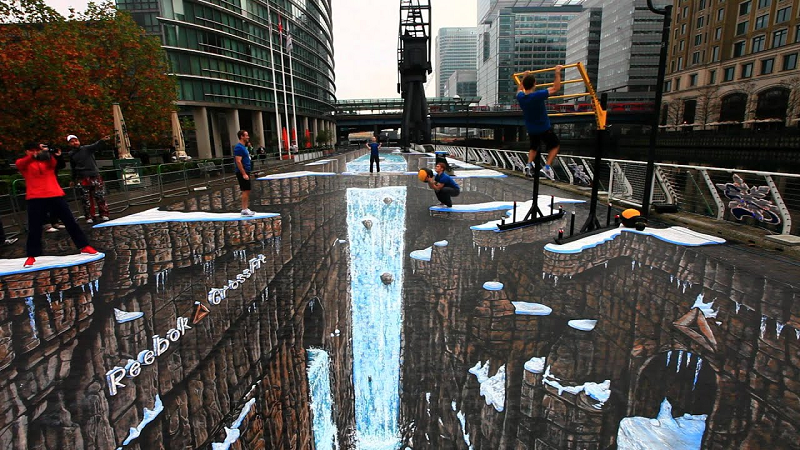
\includegraphics[width=10cm]{./figures/art3D_1.png}
\caption{2011 年最大的 3D 艺术画, 画于伦敦街头, 获吉尼斯纪录} \label{art3D_fig1}
\end{figure}

\begin{figure}[ht]
\centering
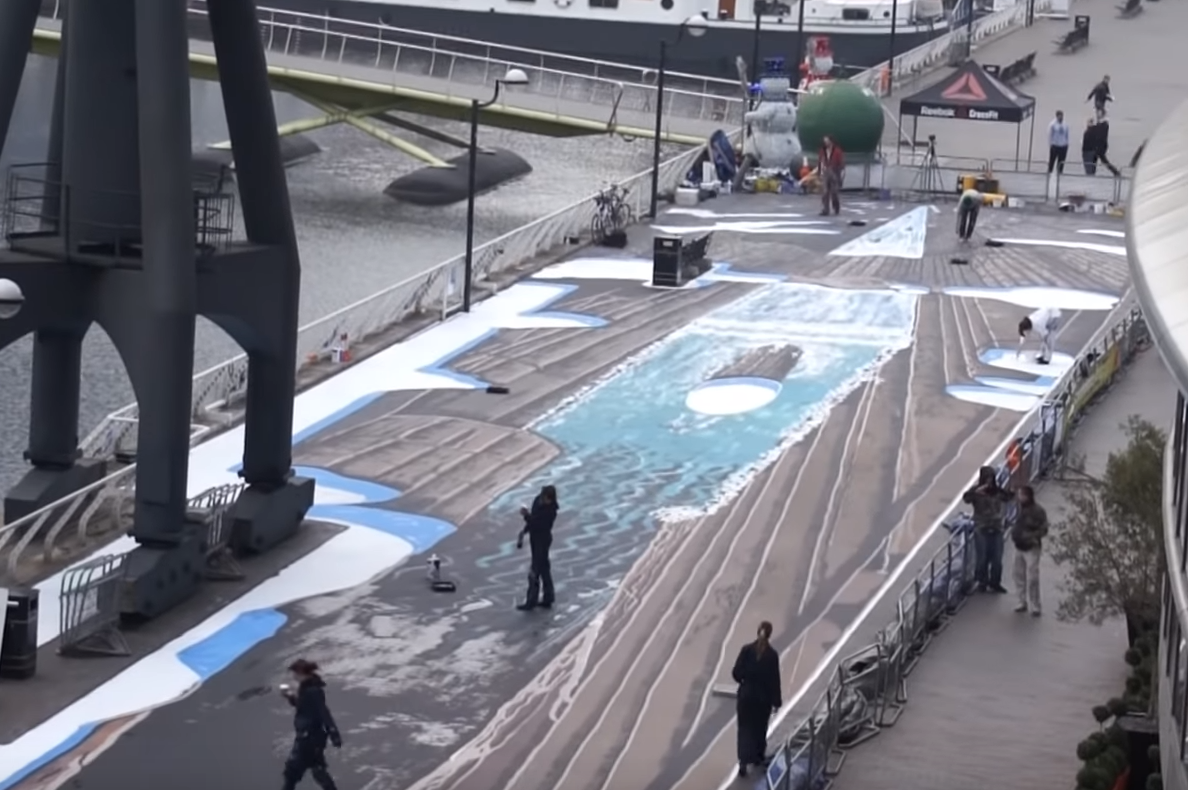
\includegraphics[width=10cm]{./figures/art3D_2.png}
\caption{从不同角度看 3D 艺术画(\autoref{art3D_fig1} 由该图中右上角相机拍摄)} \label{art3D_fig2}
\end{figure}

\subsection{计算}

\pentry{由图像坐标计算射线\upref{mn2lin}, 直线和平面的交点\upref{LPint}}

由预备知识中的两个词条, 若给出预期的效果图(即\autoref{art3D_fig1} 中的虚构部分), 世界坐标系中投影平面的位置, 以及相机模型的参数和位置, 就可以将效果图上的点一一对应到世界系的射线, 再对应到投影平面上.

我们不直接投影到世界系的 $xy$ 平面上, 是因为一些 3D 艺术画不仅使用地板, 也可能使用墙壁和天花板等多个平面.

\begin{lstlisting}[language=matlab, caption=art3D.m]
% 参数中矢量不必归一化

% === 设置相机参数 ===
imfile = 'test.png'; % 图片位置
cam_pos = [10, -10, 10]; % 世界参考系中相机位置
cam_z = -cam_pos; % 世界参考系中相机朝向
view_ang = 40/180*pi; % 相机水平视角 (单位:弧度)
cc = [0, 0]; % 光轴相对图片中心的偏移 (单位: 像素),

% === 设置投影平面 ===
plane_o = [0, 0, 0]; % 原点
plane_z = [0, 0, 1]; % z 轴单位矢量
plane_x = [1, 0, 0]; % x 轴单位矢量
% ================

% 相机坐标系
% 相机的 x 轴总是水平
cam_z = cam_z / norm(cam_z);
cam_x = cross([0, 0, -1], cam_z); cam_x = cam_x / norm(cam_x);
cam_y = cross(cam_z, cam_x);
RT = [cam_x', cam_y', cam_z']; % rotation matrix

% 平面坐标系
plane_z = plane_z / norm(plane_z);
plane_y = cross(plane_z, plane_x);
plane_y = plane_y / norm(plane_y);
plane_x = cross(plane_y, plane_z);

% 读取图片
I = imread(imfile);
[N1, N2, ~] = size(I);
f = N2/2/tan(view_ang/2); % 焦距 (单位: 像素)

% 在相机系中生成图片网格(每个像素都是网格中一个正方形)
[xc, yc] = meshgrid(linspace(0.5, N2+0.5, N2+1), linspace(0.5, N1+0.5, N1+1));
xc = xc - N2/2 + 0.5;
yc = yc - N1/2 + 0.5;

% 世界系中的射线(对应每个格点)
vc = zeros(3, (N1+1)*(N2+1));
vc(1,:) = xc(:); vc(2,:) = yc(:); vc(3,:) = f;
v = RT * vc;

% 世界系中射线与平面的交点 (参考 http://wuli.wiki/online/LPint.html)
intersec = ((plane_o - cam_pos) * plane_z') * v ./ (plane_z * v) + cam_pos';

% 将交点转换到平面参考系
inter1 = intersec - plane_o';
if max(plane_z * inter1) > 1e-14
    error('intersection not on plane');
end
xp = plane_x * inter1;
yp = plane_y * inter1;
xp = reshape(xp, N1+1, N2+1);
yp = reshape(yp, N1+1, N2+1);

% 画图
zp = zeros(size(xp));
cdata = double(I)/255; cdata(end+1, end+1, 3) = 0;
figure; surf(xp, yp, zp, 'CData', cdata, 'LineStyle', 'none');
view(0, 90); axis equal;
\end{lstlisting}
